\section{Aufbau}

Das verwendete Alibava EASy (Educational Alibava System) besteht aus den Komponenten Detektoreinheit, Kontrolleinheit und Computer.
Der Aufbau ist in Abbildung \ref{fig:aufbau} zu sehen.
\begin{figure}
  \centering
  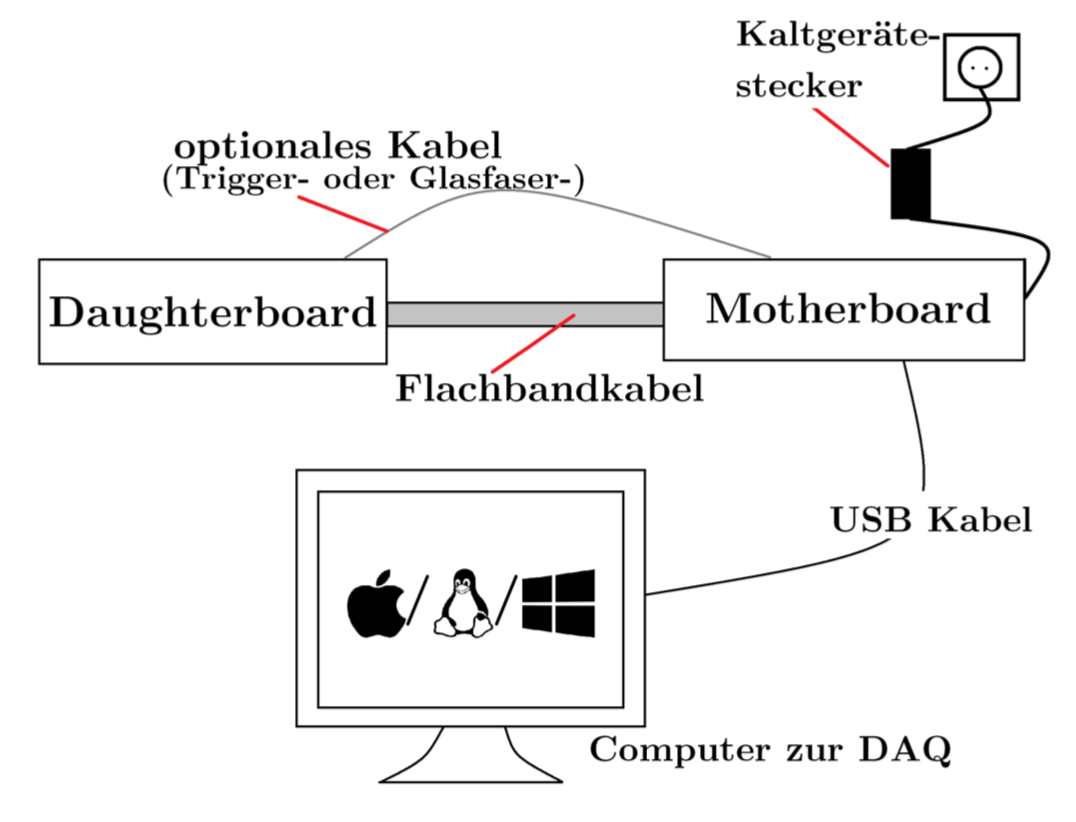
\includegraphics[height=6cm]{TimosAufrisse/aufbau.png}
  \caption{Aufbau des Alibava EASy \cite{anleitung}.}
  \label{fig:aufbau}
\end{figure}
Das Flachbandkabel zwischen Detektor- und Kontrolleinheit sorgt für die Stromversorgung und Datenübermittlung. Außerdem kann von der Kontrolleinheit an den Detektor noch ein Triggersignal gesendet. Wie sich dieses ergibt wird später noch beschrieben. Zusätzlich kann ein Laser an den Detektor angeschlossen werden, mit dem dessen Struktur untersucht wird.

\subsection{Detektoreinheit}
Der Detektor besteht aus 128 p-dotierten Streifen, die in eine $\SI{300}{\micro\meter}$ dicke n-dotierte Basis implantiert sind.
Dabei sind die Streifen einzelnd mit der Ausleseelektronik verbunden, sodass sie an einzelne Kanäle angeschlossen werden können und sich so die ortsaufgelöste Messung ergibt.
\begin{figure}
  \centering
  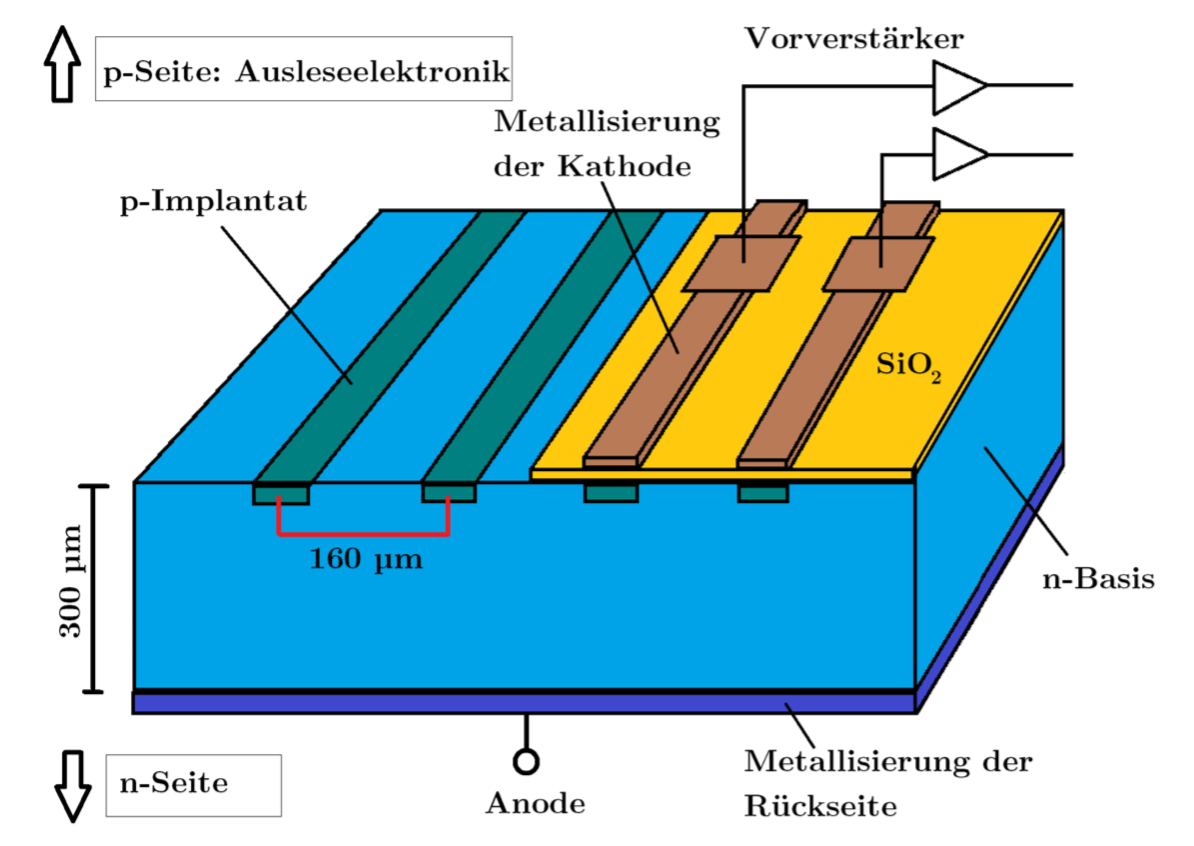
\includegraphics[height=7cm]{TimosAufrisse/detektorStreifen.png}
  \caption{Schema des Streifendetektors mit den p-dotierten Streifen und der n-dotierten Basis \cite{anleitung}.}
  \label{fig:detektorStreifen}
\end{figure}
Die Effizienz der Ladungssammlung (CCE) hängt von der angelegten Spannung $U$ an den Detektor ab und ergibt den Zusammenhang:
\begin{align}
  \text{CCE}(U) = \frac{1-\exp(\frac{-d_\text{c}(U)}{a})}{1-\exp(\frac{-D}{a})}.
  \label{eqn:cce}
\end{align}
Dabei ist $d_\text{c}(U)$ die von der Spannung abhängige Dicke der Depletionszone, $a$ die Eindringtiefe des zur Messung genutzten Lasers und $D = \SI{300}{\micro\meter}$ die Dicke des Detektors.

\subsection{Laser}
Der zur Vermessung des Detektors genutzte Laser hat eine Wellenlänge von $\SI{980}{\nano\meter}$ und bedeckt eine Fläche von $\SI{20}{\micro\meter}$ im Durchmesser auf dem Detektor. Seine Spitzenleistung beträgt $\SI{0.6}{\milli\watt}$ bei einer Pulslänge von $\SI{5}{\nano\second}$. Seine Position über dem Detektor lässt sich horizontal und vertikal mit Mikrometerschrauben verstellen.

\subsection{Kontrolleinheit}
An der Kontrolleinheit lässt sich die Spannung, die am Detektor anliegt, einstellen und der fließende Strom ablesen. Außerdem liefert sie den Laser und verarbeitet das Triggersignal. Das Triggersignal wird dabei durch eine Diode erzeugt, die unter dem Streifendetektor angebracht ist und nur dann ein Signal liefert, wenn die einfallende Strahlung genug Energie besitzt um den eigentlichen Detektor zu durchdringen und dann auch in der Diode Energie deponiert. Eine Skizze dieses Aufbaus ist in Abbildung \ref{fig:diodenTrigger} zu sehen.
\begin{figure}
  \centering
  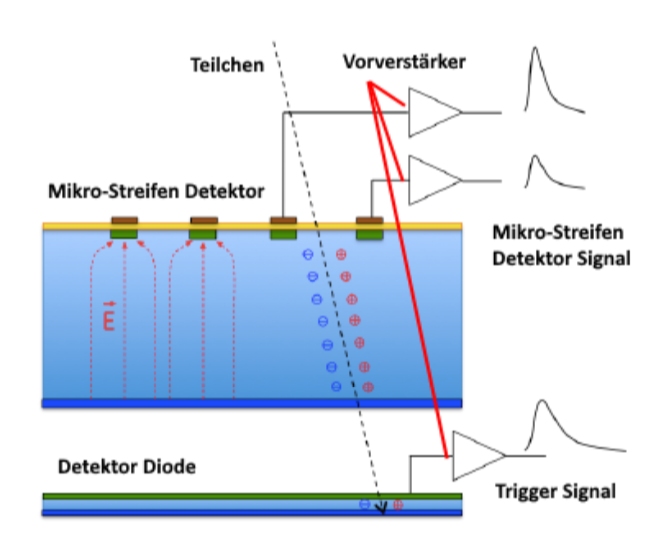
\includegraphics[height=7cm]{TimosAufrisse/diodenTrigger.png}
  \caption{Die Diode als Trigger \cite{anleitung}.}
  \label{fig:diodenTrigger}
\end{figure}
Das Triggersignal sorgt also dafür, dass nur die Daten aufgenommen werden, die von interessantent Elektronen stammen, da niederenergetischer Background so reduziert wird.

\subsection{Computer}
Die Kontrolleinheit wird per USB-Kabel an den Computer angeschlossen. An diesem können mit der Alibava gui Einstellungen vorgenommen werden. Außerdem werden dort die Daten gespeichert und mit einem Auswärteskript vorprozessiert.




 \section{Durchführung}
\label{sec:Durchführung}

\subsection{Messung der Strom-Spannungs-Kennlinie}
Zur Aufnahme einer Strom-Spannungs-Kennlinie wird die Spannung, die am Detektor anliegt, an der Kontrolleinheit in \SI{10}{\volt}-Schritten in dem Bereich \SI{0}{\volt} bis \SI{200}{\volt} geregelt. Dazu ist mit der Anzeige zu jedem Spannungswert ein Wert für den Leckstrom aufzunehmen.

\subsection{Pedestals und Noise}
Um den Offset und den Common Mode Shift aufzunehmen wird ein \textit{Pedestal Run} mit 1000 Events durchgeführt.

\subsection{Kalibration}
Mit einem \textit{Delay Scan} wird zunächst die optimale Verzögerung zwischen Signal und Auslese bestimmt. Nach dem Eintragen des so ermittelten Werts ins Kalibrationsfenster wird eine Kalibrationskurve für fünf Kanäle bei $U > U_\text{dep}$ aufgenommen. Eingestellt wird dabei der \textit{Calibration Run}. Diese Messung wird dann nochmal bei einem Kanal mit $U=\SI{0}{\volt}$ wiederholt.

\subsection{Sensorvermessung mittels Laser}
Für diesen Teil wird der Laser an den Detektor angeschlossen.
Zunächst wird auch hier die optimale Verzögerung zwischen Signal und Auslese bestimmt.
Dann wird der Laser in $\SI{10}{\micro\meter}$ großen Schritten auf 35 Punkte gefahren und je eine Messung mit 1000 Events durchgeführt.

\subsection{Bestimmung der Charge Collection Efficiency}
\paragraph{Mit Laser:}
Um die Effizienz des Detektors in Korrelation zur angelegten Spannung zu untersuchen, wird die Spannung erneut in $\SI{10}{\volt}$-Schritten in dem Bereich \SI{0}{\volt} bis \SI{200}{\volt} erhöht. Zu jeder Spannung wird dann bei verbundener Lasereinheit eine Messung mit 1000 Events durchgeführt.
\paragraph{Mit $\beta^-$-Quelle:}
\begin{figure}
  \centering
  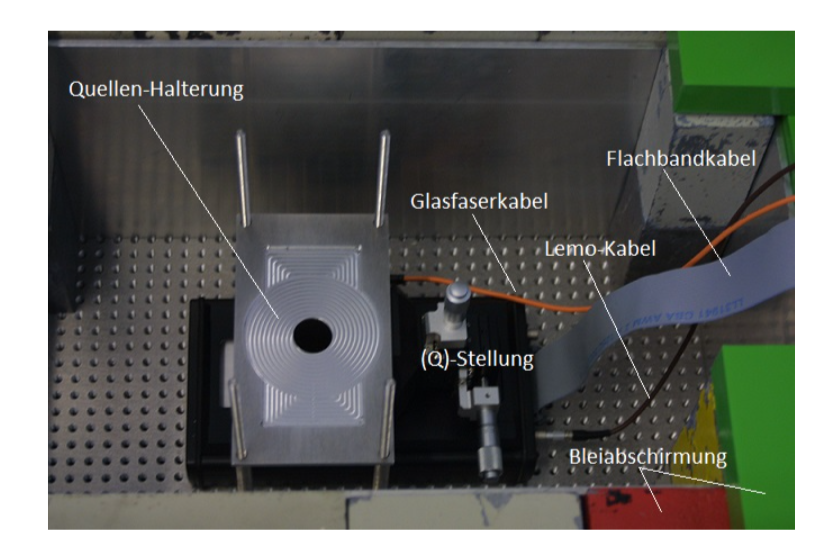
\includegraphics[height=7cm]{TimosAufrisse/quellenmessung.png}
  \caption{Der Detektor bei Aufnahme der Messwerte einer $\beta^-$-Quelle \cite{anleitung}.}
  \label{fig:quellenmessung}
\end{figure}
Hier wird der Detektor wie in Abbildung \ref{fig:quellenmessung} gezeigt verkabelt. Die Spannung wird erneut wie bei der CCE-Bestimmung mit dem Laser geregelt und es werden \num{10000} Events aufgenommen.

\subsection{Großer Quellenscan}
Zuletzt wird mit dem Quellenaufbau noch ein \textit{RS Run} mit $\num{1e6}$ Events durchgeführt.
